\documentclass[11pt, onecolumn, compsoc, letterpaper]{article}

% Usual setup packages
\usepackage{times}
\usepackage[utf8]{inputenc} % set input encoding (not needed with XeLaTeX)
\usepackage[margin=2.75cm]{geometry} % to change the page dimensions
\usepackage{graphicx} % General page control package
\usepackage[compact]{titlesec} % For compact title
\usepackage{listings} % For including source code with highlighting
\usepackage{hyperref} % For better hyper-link integration

% Packages for verbatim text blocks
\usepackage{alltt} % Package for including math in verbatim text
\usepackage{fancyvrb}

% Packages for math symbols and other mathey things
\usepackage{amsmath}
\usepackage{amsfonts}
\usepackage{amssymb}
\usepackage{mathtools}

% Packages for including pseudo-code
\usepackage{algorithmicx}
\usepackage{algorithm}
\usepackage{algpseudocode}

% Packages that handle lists
\usepackage{enumerate} % For reduced enumeration spacing
%\usepackage{enumitem} % For suppressing bullets
\usepackage{mdwlist} % Better control of lists

% Packages that handle tables, figures and other floats
\usepackage{tabularx}
\usepackage{multirow}
\usepackage{titling}
\usepackage{float} % To make floats movable
\usepackage[font=scriptsize,labelfont=bf]{caption}
\usepackage[font=scriptsize,labelfont=bf]{subcaption}
\usepackage{hhline}
\usepackage[usenames,dvipsnames]{color}
\usepackage[table]{xcolor}

% Packages for drawing graphs, FSMs, etc.
\usepackage{pgf}
\usepackage{tikz}
\usepackage{tikz-qtree}
\usetikzlibrary{shapes,arrows,calc,fit,positioning,shapes.symbols,shapes.callouts,patterns,automata}

% clean up references
\hypersetup{
    colorlinks,
    citecolor=black,
    filecolor=black,
    linkcolor=black,
    urlcolor=black
}

% smaller tab space
\lstset{tabsize=4}

%%% HEADERS & FOOTERS
\usepackage{titlepic}
\usepackage{fancyhdr} % This should be set AFTER setting up the page geometry
\pagestyle{fancy} % options: empty , plain , fancy
\renewcommand{\headrulewidth}{0pt} % customise the layout...
\lhead{}\chead{}\rhead{}
\lfoot{}\cfoot{\thepage}\rfoot{}

%%% SECTION TITLE APPEARANCE
%\usepackage{sectsty}
%\allsectionsfont{\sffamily\mdseries\upshape} % (See the fntguide.pdf for font help)
% (This matches ConTeXt defaults)

%%% ToC (table of contents) APPEARANCE
%\usepackage[nottoc,notlof,notlot]{tocbibind} % Put the bibliography in the ToC
%\usepackage[titles,subfigure]{tocloft} % Alter the style of the Table of Contents
%\renewcommand{\cftsecfont}{\rmfamily\mdseries\upshape}
%\renewcommand{\cftsecpagefont}{\rmfamily\mdseries\upshape} % No bold!

% Nice Little macro for adding a comment box. Includes incrementing comment numbers.
\newcounter{comcount}
\setcounter{comcount}{0}
\newcommand{\mycomment}[1]
{
\refstepcounter{comcount}
\textcolor{red}{\textbf{\emph{\arabic{comcount}}: \small{#1}}}
}

% Math commands
\newcommand{\edit}[1]{\textcolor{red}{#1}}

\newcommand{\vnorm}[1]{\left|\left|#1\right|\right|}
\newcommand{\tab}{\hspace*{2em}}
\DeclareMathOperator*{\argminop}{arg\,min\,}
\DeclareMathOperator*{\argmaxop}{arg\,max\,}
\DeclarePairedDelimiter\ceil{\lceil}{\rceil}
\DeclarePairedDelimiter\floor{\lfloor}{\rfloor}
\newcommand{\argmin}[1]{\underset{#1}{\argminop}}
\newcommand{\argmax}[1]{\underset{#1}{\argmaxop}}
\newcommand{\D}[2]{\frac{d#1}{d#2}}
\newcommand{\PD}[2]{\frac{\partial #1}{\partial #2}}
\newcommand{\V}[1]{\mathbf{#1}}
\newcommand{\ubar}[1]{\underline{#1}}
\newcommand{\Sig}{\mathcal{S}}  % Sigmoid function
\newcommand{\Pl}{\mathcal{N}} % Player List
\newcommand{\Ta}{\mathcal{T}} % Targets/Resources
\newcommand{\We}{\mathcal{W}} % (All) Global Welfare Function

% Squeeze whitespace
\setlength{\parskip}{0pt}
\setlength{\parsep}{0pt}
\setlength{\headsep}{0pt}
\setlength{\topskip}{0pt}
\setlength{\topmargin}{0pt}
\setlength{\topsep}{0pt}
\setlength{\partopsep}{0pt}

\titlespacing{\section}{0pt}{*3}{*3}
\titlespacing{\subsection}{0pt}{*2}{*2}
\titlespacing{\subsubsection}{0pt}{*1}{*1}

\renewcommand{\arraystretch}{1.2}
\setlength{\droptitle}{-2cm}

\title{Performance Bounds on Centralized vs.~Distributed Task Allocation with Constraints}
\author{Anshul Kanakia, Nikolaus Correll}
\date{}

\begin{document}
\maketitle

\begin{abstract}
Task allocation is a well studied problem in the fields of robotics, optimization, and game theory where a number of identical agents must be assigned to the a number of collaborative tasks for maximum system welfare. Swarm robotics in particular has tackled this problem for a number of years and many centralized, distributed, and hybrid approaches exist for solving task allocation. Practical deployment of multi-agent systems for automated surveillance, robotic firefighting, and oil-spill containment among other tasks has been proposed as a viable alternative to existing approaches and corresponding task allocation strategies for each of these applications have been analyzed but there has so far been no formal unifying definition for optimal task allocation in swarm robotics. This paper therefore presents a formal problem definition for multi-agent task allocation as well as a general definition of optimal task allocation. A centralized approach is then compared as a baseline optimum to a proposed distributed task allocation method. The distributed method is an extension of existing work done using response threshold algorithms. While a centralized approach to task allocation is always optimal when provided with perfect information about the real-world system, in realistic scenarios involving agent and task constraints and imperfect sensing and communication we see that the distributed approach quickly attains a comparable level of performance and should be the preferred method of deployment due to the advantages it provides in reliability and robustness to agent level failure.
\end{abstract}

\section{Introduction}
Task allocation (TA) is ubiquitous in different fields of research. It is often called task allocation or task assignment in the field of robotics, specifically, swarm robotics and multi-agent systems (MAS). An equivalent problem is studied by ethologists to model division of labor in social insect colonies. In theoretical computer science there is a generalized formulation of task allocation called the multiple integer knapsack problem. In game theory, this problem is referred to as the vehicle-target assignment problem. Each of these formulations provides a unique perspective for studying the same problem and leveraging these different perspectives is essential for providing a generalized definition for TA. 

As pointed out in \cite{gerkey2004formal}, while the research areas of MAS and TA have expanded considerably over the last decade most of the work on multi-agent task allocation (MATA) has focused mainly on very specific proof-of-concept examples of MATA system design. Even ten years later, current TA models are for scenarios such as foraging or surveillance or containment and service a niche in the domain. There is as yet no general model for MATA that can be used to globally define the problem. Gerkey et al.~\cite{gerkey2004formal}, provide an excellent starting point for this. The paper categorizes existing work in the field while also providing a utility based definition for MATA optimality but does not present a generalized MATA model. While Gerkey et al.~\cite{gerkey2004formal} provide a taxonomy of existing MATA architectures, our goal with this paper is to provide a much more general low-level model for MATA and propose a definition of optimality that holds true under most specific TA scenarios. We do not provide a comparison of existing models in the field but instead attempt to situate our proposed general model for MATA as a valid framework that both existing and new  architectures can be molded to fit within. 

\subsection{Related Work}

\section{Problem Definition and Example}
TA is a canonical problem in swarm robotics. With the advent of more sophisticated general purpose robots such as the Baxter, NAO and innumerable UAVs the problem of handling real world tasks collaboratively, be it with other robots or humans, is becoming increasingly important. Many group tasks exhibit a property of concurrent benefit, i.e. single agent attempts to complete the task are guaranteed to fail or waste resources but groups attempting the task together provide a considerable concurrency benefit. A problem oft ignored by MATA model developers is deciding when a group is capable enough to attempt the collaborative task and whether or not simultaneous actions are important to complete the task successfully. While this precise temporal component of attempting tasks concurrently is not the focus of our work, it is important to point out as we make certain assumptions on required task group sizes and how these requirements change with time. In this context TA is distilled down to the process of assigning the required number of agents to particular dynamic tasks without worrying about how agents get to the tasks or what the exact dynamics of agents and these genericized tasks are. 

We assume that tasks or targets (used synonymously throughout this paper) require at least two agents to attempt collaboratively. The major caveat here is that the \emph{exact} number of agents required to attempt a task is unknown and very difficult to accurately discern. Tasks with concurrent benefit share the property that the probability of success depends non-linearly on the collective capabilities and team size of the robots attempting it. In addition, the exact number of agents required to successfully complete the task varies over time due to numerous  complex physical parameters. Many collaborative tasks---particularly those seen in biological systems---exhibit the property of concurrent benefit, ranging from surveillance and coordinated defense of enclosed areas like termite mounds and honey bee hives \cite{breed1990division} to collective transport of heavy objects and even containment of oil spills and forest fires. To contain a large fire, it is insufficient (and inefficient) for a single agent to start putting out the fire without waiting for backup. But the rate of fire containment increases quickly by adding just a few more agents to the group, which illustrates the property of concurrent benefit well.

\subsection{Multi-Agent Task Allocation Model}
With this general overview of MATA in mind, we present the following formal model for TA.
\begin{itemize}
	\item Agents/Players: $\Pl = \{n_1, n_2, \ldots, n_i, \ldots,n_{|\Pl|}\}$
	\item Targets: $\Ta = \{t_1, t_2, \ldots, t_j, \ldots,t_{|\Ta|}\}$
	\item Target Threshold: $K:\Ta \to \mathbb{Z}^+$\\
	The number of agents required to successfully attempt task-$t_j$ is $= K(t_j)$, which is shortened to $k_j$ for brevity.
	
	\item Agent Constraints: $C:\Pl \to \hat{\Ta} \subseteq \Ta$\\
	The set of constraints for agent-$n_i$ ($= C(n_i)$) is the subset of targets that this agent can reach. It is shortened to $c_i$ for brevity.
	\item Agent Assignment Matrix: A $|\Pl| \times |\Ta|$ matrix of 0-1 elements $x(n_i, t_j)$ or $x_{ij}$ for short, that are either $0$ if agent-$i$ is not assigned to target-$j$ or $1$ if agent-$i$ is assigned to target-$j$.
	\begin{equation}\label{eq:X}
		X = \left(\begin{array}{ccc}
			x_{11} & \ldots & x_{1|\Ta|}\\
			\vdots & \ddots & \vdots\\
			x_{|\Pl|1} & \ldots & x_{|\Pl||\Ta|}
		\end{array}\right)
	\end{equation}
	\item Target Assignments: $A:\Ta \to \hat{\Pl} \subseteq \Pl$\\
	The set of agents assigned to target-$t_j$ is $= A(t_j)$, which is shortened to $a_j$ for brevity. From~\eqref{eq:X} we can define
\begin{equation}\label{eq:aj}
	|a_j| = \sum\limits_{i = 1}^{|\Pl|} x_{ij}
\end{equation}
	\textbf{Definition:} A target is considered ``successfully assigned'' when $|a_j| \geq k_j$, i.e. the number of player's assigned to it is greater than or equal to its threshold value.\\
	\textbf{Definition:} A target is considered ``perfectly assigned'' when $|a_j| = k_j$.
	\item Target specific welfare function,
\begin{align}\label{eq:wf}
	W(t_j, |a_j|) & = \left\{
	\begin{array}{ll}
		w_j & |a_j| \geq k_j\\
		0 & o/w
	\end{array}\right.
\end{align}
where $w_j$ can be a value or function defining the utility of completing task-$t_j$ upon successful assignment.

	\item Global welfare function,
\begin{align}\label{eq:gwf}
	\We = \sum\limits_{j = 1}^{|\Ta|} W(t_j, |a_j|)
\end{align}
\end{itemize}

Eqn.~\eqref{eq:gwf} is an objective function that can be maximized to provide an \emph{optimal} assignment of agents to targets. This is in contrast to a lot of existing approaches for MATA where each agent is concerned with maximizing their own utility, making such approaches agent-centric. We, instead, focus on the task as the primary entity for which a utility function is defined and maximized. This approach falls more in line with work such as \cite{shehory1998methods}.

\subsection{Defining Optimality for Multi-Agent Task Allocation}
Consider a simplified forest firefighting scenario where a number of isolated fires and flame fronts exist in a specified geographic region. Our goal is to contain all of the fires and prevent them from spreading or, at the very least, contain as many as we can given our manpower. If the fires did not evolve over time and we had perfect information about the threshold value of each target/fire then a central controller would only have to maximize Eqn.~\eqref{eq:gwf} subject to the constraints mentioned in Table~\ref{tab:constraints} and provide the resulting assignment matrix to all the agents. The agents would then move to their assigned fires. Since Eqn.~\eqref{eq:gwf} guarantees successful assignments (if such an assignment is possible) there would be enough robots at each fire to put it out and all the tasks would be complete. 

Clearly this situation --- like most real world situations --- is dynamic, i.e., the size and number of fires changes over time. The task allocation model described in the previous section has no notion of time. We consider constant but repeated optimization of ``snapshots'' of a dynamic problem so that at any given point a solution to the TA problem is valid. The main assumption made here is that maximizing Eqn.~\eqref{eq:gwf} subject to the constraints listed in Table~\ref{tab:constaints} takes considerably less time than the physical evolution of the task magnitudes, and in-turn, the task thresholds. If this is not the case or if, for any other reason, the state of the system is not updated in a central controller then this notion of optimality quickly fails.

Nevertheless, maximizing snapshots of a MATA system with perfect information throughout the course of a prescribed scenario provides a means for defining baseline system-wide optimality. At any given point in time, the optimal solution of a snapshot of the state of the system is the best assignment of targets that agents can be given.

\edit{I fully expect the reader to still have a number of questions about the notion of optimality here and perhaps the fact that a formal definition of optimal TA is still missing is a deal-breaker for this section but nevertheless, the discussion above is important to convey the context of this problem.} 

\subsection{Example}
The following example describes a cooperative game with target thresholds and player constraints as seen in Figure \ref{fig:ex1}.
\begin{itemize}
	\item Agent: $\Pl = \{1,2,3,4\}$
	\item Targets: $t \in \Ta = \{a, b, c\}$
	\item Target thresholds: $k_a = k_b = k_c = 2$
	\item Agent constraints: $c_1 = c_3 = \{a, b\}$ and $c_2 = c_4 = \{b, c\}$
	\item Target specific welfare function: $W(t_j, |a_j|) = 1$ (if $|a_j| \geq k_j$), $0$ otherwise.
	
\end{itemize}
\begin{figure}[!htb]
	\centering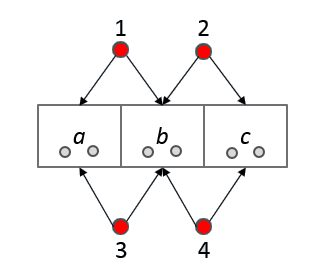
\includegraphics[width=5.5cm]{assets/ex1.png}
	\centering\caption{A cooperative game with 4 players and 3 targets. Gray pegs indicate the target's minimum threshold value while the arrows depict player assignment constraints.}\label{fig:ex1}
\end{figure}

\section{Centralized vs.~Distributed Task Allocation}
\subsection{Centralized Task Allocation Strategy}
\subsection{Distributed Task Allocation Strategy}
\subsection{Comparative Analysis}
\section{Experiment Setup}
\subsection{Centralized Task Allocation Experiments}
\subsection{Distributed Task Allocation Experiments}
\section{Results}
\section{Analysis and Discussion}
\section{Conclusion}

\bibliographystyle{plain}
\bibliography{refs}

\end{document}